\begin{figure}[H]
\centering
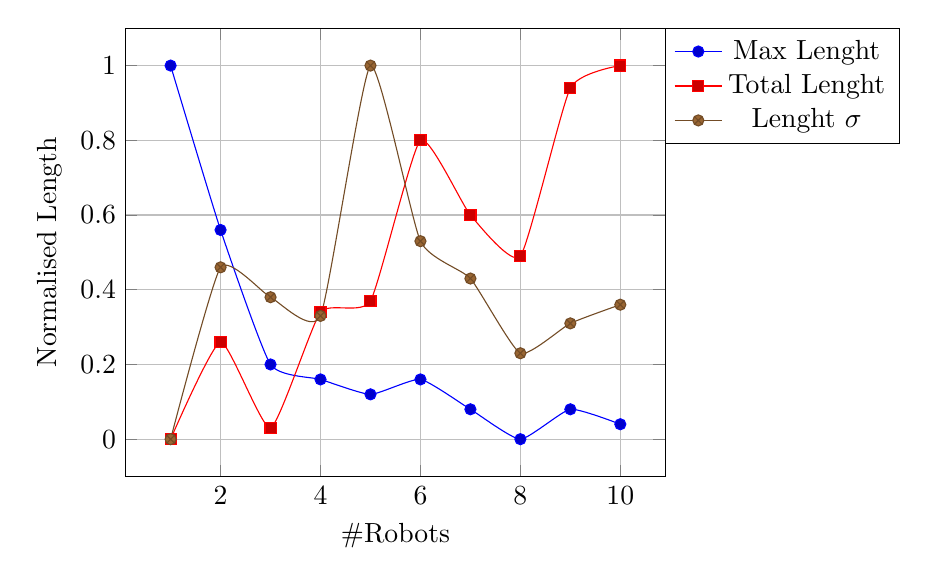
\begin{tikzpicture}
	\begin{axis}[
%		height=9cm,
%		width=9cm,
		grid=major,
                legend style = {at={(1,1)}, anchor=north west},
		xlabel=\#Robots,
		ylabel=Normalised Length,
		smooth,
		tension=0.3
	]

	\addplot coordinates {
(1, 1.00)
(2, 0.56)
(3, 0.20)
(4, 0.16)
(5, 0.12)
(6, 0.16)
(7, 0.08)
(8, 0.00)
(9, 0.08)
(10, 0.04)
	};
	\addlegendentry{Max Lenght}

	\addplot coordinates {
(1, 0.00)
(2, 0.26)
(3, 0.03)
(4, 0.34)
(5, 0.37)
(6, 0.80)
(7, 0.60)
(8, 0.49)
(9, 0.94)
(10, 1.00)
	};
	\addlegendentry{Total Lenght}

	\addplot coordinates {
(1, 0.00)
(2, 0.46)
(3, 0.38)
(4, 0.33)
(5, 1.00)
(6, 0.53)
(7, 0.43)
(8, 0.23)
(9, 0.31)
(10, 0.36)
	};
	\addlegendentry{Lenght $\sigma$}
	\end{axis}
\end{tikzpicture}
\caption{Variation of the performance indexes increasing the number of robots, for the 5x5 grid using the LRTA* algorithm}
\end{figure}